\documentclass[11pt, oneside]{article}   	% use "amsart" instead of "article" for AMSLaTeX format
\usepackage{geometry}                		% See geometry.pdf to learn the layout options. There are lots.
\geometry{letterpaper}                   		% ... or a4paper or a5paper or ... 
%\geometry{landscape}                		% Activate for rotated page geometry
%\usepackage[parfill]{parskip}    		% Activate to begin paragraphs with an empty line rather than an indent
\usepackage{graphicx}				% Use pdf, png, jpg, or eps§ with pdflatex; use eps in DVI mode
								% TeX will automatically convert eps --> pdf in pdflatex		
\usepackage{amssymb}

\usepackage{amsmath}
%SetFonts

%SetFonts


\title{Algorand Independent Work Updates}
\author{Jason Shi}
%\date{}							% Activate to display a given date or no date

\begin{document}
\maketitle
\section{Update 1: Preliminary Work}
\subsection{Framing the Problem}

The goal of the project is to describe $F(x)$ where $F(x)$ is the fraction of rewards you can get with owning a fraction $x$ of the wealth.

\subsection{Setup and Definitions}
\begin{itemize}
  \item Let there be $K$ coins in total.
  \item $P_{k, x}$ is the probability that you own the top $k$ coins but not the $k+1$-th coin, given that you own a fraction $x$ of the wealth. Note that this depends on $K$, the total number of coins.
\end{itemize}

\subsection{Initial Steps}

First define $F_1(x)$ as the fraction of the rewards you can get with owning a fraction $x$ of the wealth if the strategy is as follows. Every odd numbered round, you play to maximize the probability of winning the reward in the subsequent round. This is the very naive strategy that I believe we had talked about during our first meeting.

I recall from our first meeting that you suggested the answer to this problem is of the form

$$
F_1(x) = \sum_{k=1}^{\infty} P_{k, x} \left(\frac{kx}{kx+1-x}\right)
$$

where $P_{k, x}$ is the probability of owning the top $k$ coins but not the $(k+1$)-th coin, given owning a fraction $x$ of the wealth. We define the top $k$ coins as the first $k$ coins in following list that spans all $K$ coins $\{c_i\}_{i=1}^K$,

$$
L = \{H(SIG_{owner(c_i)}(seed_r), c_i)\}_{i=1}^K
$$

such that this list is in ascending order. That is, coins that appear earlier on this list beat coins that appear later on the list in the Algorand consensus.

I do not quite recall the reasoning behind the above expansion for $F_1(x)$, but I have arrived at a different expression using the following approach. If you own the top $k$ coins, then you can guarantee winning the first round and reward $1$ if you choose to transmit any of these $k$ coins, and each coin gives you an independent probability $x$ of winning the next round. Assume that winning this round is better for you than losing this round, which is intuitively true but not yet proven. Then the probability you win the next round is the complement of the probability you lose the next round for each $k$ coins you transmit, which is $(1-x)^k$, so the overall probability is $1-(1-x)^k$. So in the first round, you win $1$ reward, and in the second round the expected reward is $1-(1-x)^k$. So, you can repeat this strategy completely from the start of every odd round. So this in this two round scenario, the fraction of reward you win is

\begin{align*}
F_1(x) &= \frac12P_{0, x}(0 + x) + \frac12\sum_{k=1}^{K} P_{k, x} \left(1+1-(1-x)^k \right) \\
& = \frac{x}2P_{0,x} +  x -  \frac12\sum_{k=1}^{K} P_{k, x} (1-x)^k 
\end{align*}

As a sanity check, after some algebra we see this is indeed greater than $x$, which is the fair fraction of the rewards you should get without performing any special strategy. So employing this naive strategy indeed increases your fraction of the rewards.

\subsection{Formulating the General Problem}
In general, the optimal play is not to only look one round ahead, but optimize over the future. That is, denote $F(x)$ be the maximum expected share of the rewards you can win by owning a fraction $x$ of the wealth. Let $F(x, k)$ be the maximum expected share of the rewards you can win by owning a fraction $x$ of the wealth given that you own the top $k$ coins, as defined above. Then we necessarily have the following equalities.

\begin{align*}
F(x) &= \sum_{k=0}^K P_{k, x} F(x, k)
\end{align*}

\begin{align*}
F(x, k) &= \sum_{i=0}^K \left[\left(\sum_{j=0}^i P_{j, x}\right)^k - \left( \sum_{j=0}^{i-1} P_{j, x} \right)^k\right]F(x, i)
\end{align*}

The first equality arises from the expansion of all the possible cases $k$ where you own the top $k$ coins. That is, you own the top $k$ coins with probability $P_{k, x}$. But if you own the top $k$ coins, then the maximum expected share of the rewards you can win is just $F(x, k)$.

The second equality arises from a similar expansion of outcomes. We consider all possible cases for the next round. That is, consider the case where in the second round, the most number of coins you can own is the top $i$ coins. This occurs with probability $\left(\sum_{j=0}^i P_{j, x}\right)^k - \left( \sum_{j=0}^{i-1} P_{j, x} \right)^k$ because you own at most the top $i$ coins with probability $\sum_{j=0}^i P_{j, x}$ but you get $k$ tries for this to happen so you raise this probability to the $k$-th power as each try is independent. But then you want to guarantee you get the top $i$ and nothing less so you subtract the probability you only get the top $i-1$ coins. So in this case you can get an expected share $F(x, i)$ of the rewards from the second round onwards. You can disregard the reward you won from the first round because we are averaging across all time, so the first round's contribution is negligible $\leftarrow$ is this rigorous?

\subsection{Some Questions}
\begin{itemize}
  \item First, I don't understand how we can order the list $L = \{H(SIG_{owner(c_i)}(seed_r), c_i)\}_{i=1}^K$ in the first place. In order for you to know that you have the top $k$ coins, then you must be able to compute $H(SIG_{owner(c_i)}(seed_r), c_i)$ for each coin $c_i$. But this involves first knowing the owner, $owner(c_i)$, of each coin, which is possible given a record of previous transactions. But this also requires computing $SIG_{owner(c_i)}(seed_r)$, which involves knowing the outcome of the owner signing the seed. I am not sure how this is possible because you need the owner's private key in order to sign the seed, that is, only the owner should be able to sign the seed.
  \item Likewise, in order to see how many top coins you have in the subsequent round, you must also be able to compute the signature of all the coins in the subsequent round as well, but only the owner of each coin has access to their own signature function.
  \item Next, can we assume that every single coin is proposed in Algorand? That is, is it only possible to win the round if you have the first coin in list $L$?
  \item Along with the previous question, is it always true that the first coin in the list $L$ is guaranteed to win? So during the gossip round of Algorand, the first coin in $L$ is propagated and enough players take it so that it is agreed during the Byzantine Consensus phase?
\end{itemize}

\section{Update 2: Corrected Approach?}

\subsection{What Went Wrong?}
Essentially, math from last update was wrong because adversary can't guarantee that he will win subsequent rounds, but the adversary can only know the probability that he will win. The previous analysis assumes that adversary can choose the world that guarantees his win.

\subsection{New Approach}
We define a subgame as follows. The Algorand algorithm is run for a constant finite $n$ number of times. Assume the adversary employs the strategy to maximize his expected overall reward, then we can calculate the adversary's expected total reward from playing the game for $n$ rounds. The hope is to take the limit of this reward divided by $n$ as $n\rightarrow \infty$ to estimate $F(x)$.

\subsubsection{Notation}
Let $F_n(x)$ denote the expected total reward from the adversary's strategy on an $n$ round game. Let the function $Reward^{(n)}_{r}(c_i)$ denote the expected total future reward that the adversary will win starting with round $r$ in an $n$ round subgame if he wins with coin $c_i$ in the previous round. Thus, this expectation is conditioned on him winning the previous round and therefore knows the seed and hashes of all his coins in the immediate subsequent round.


\begin{figure}
\centering
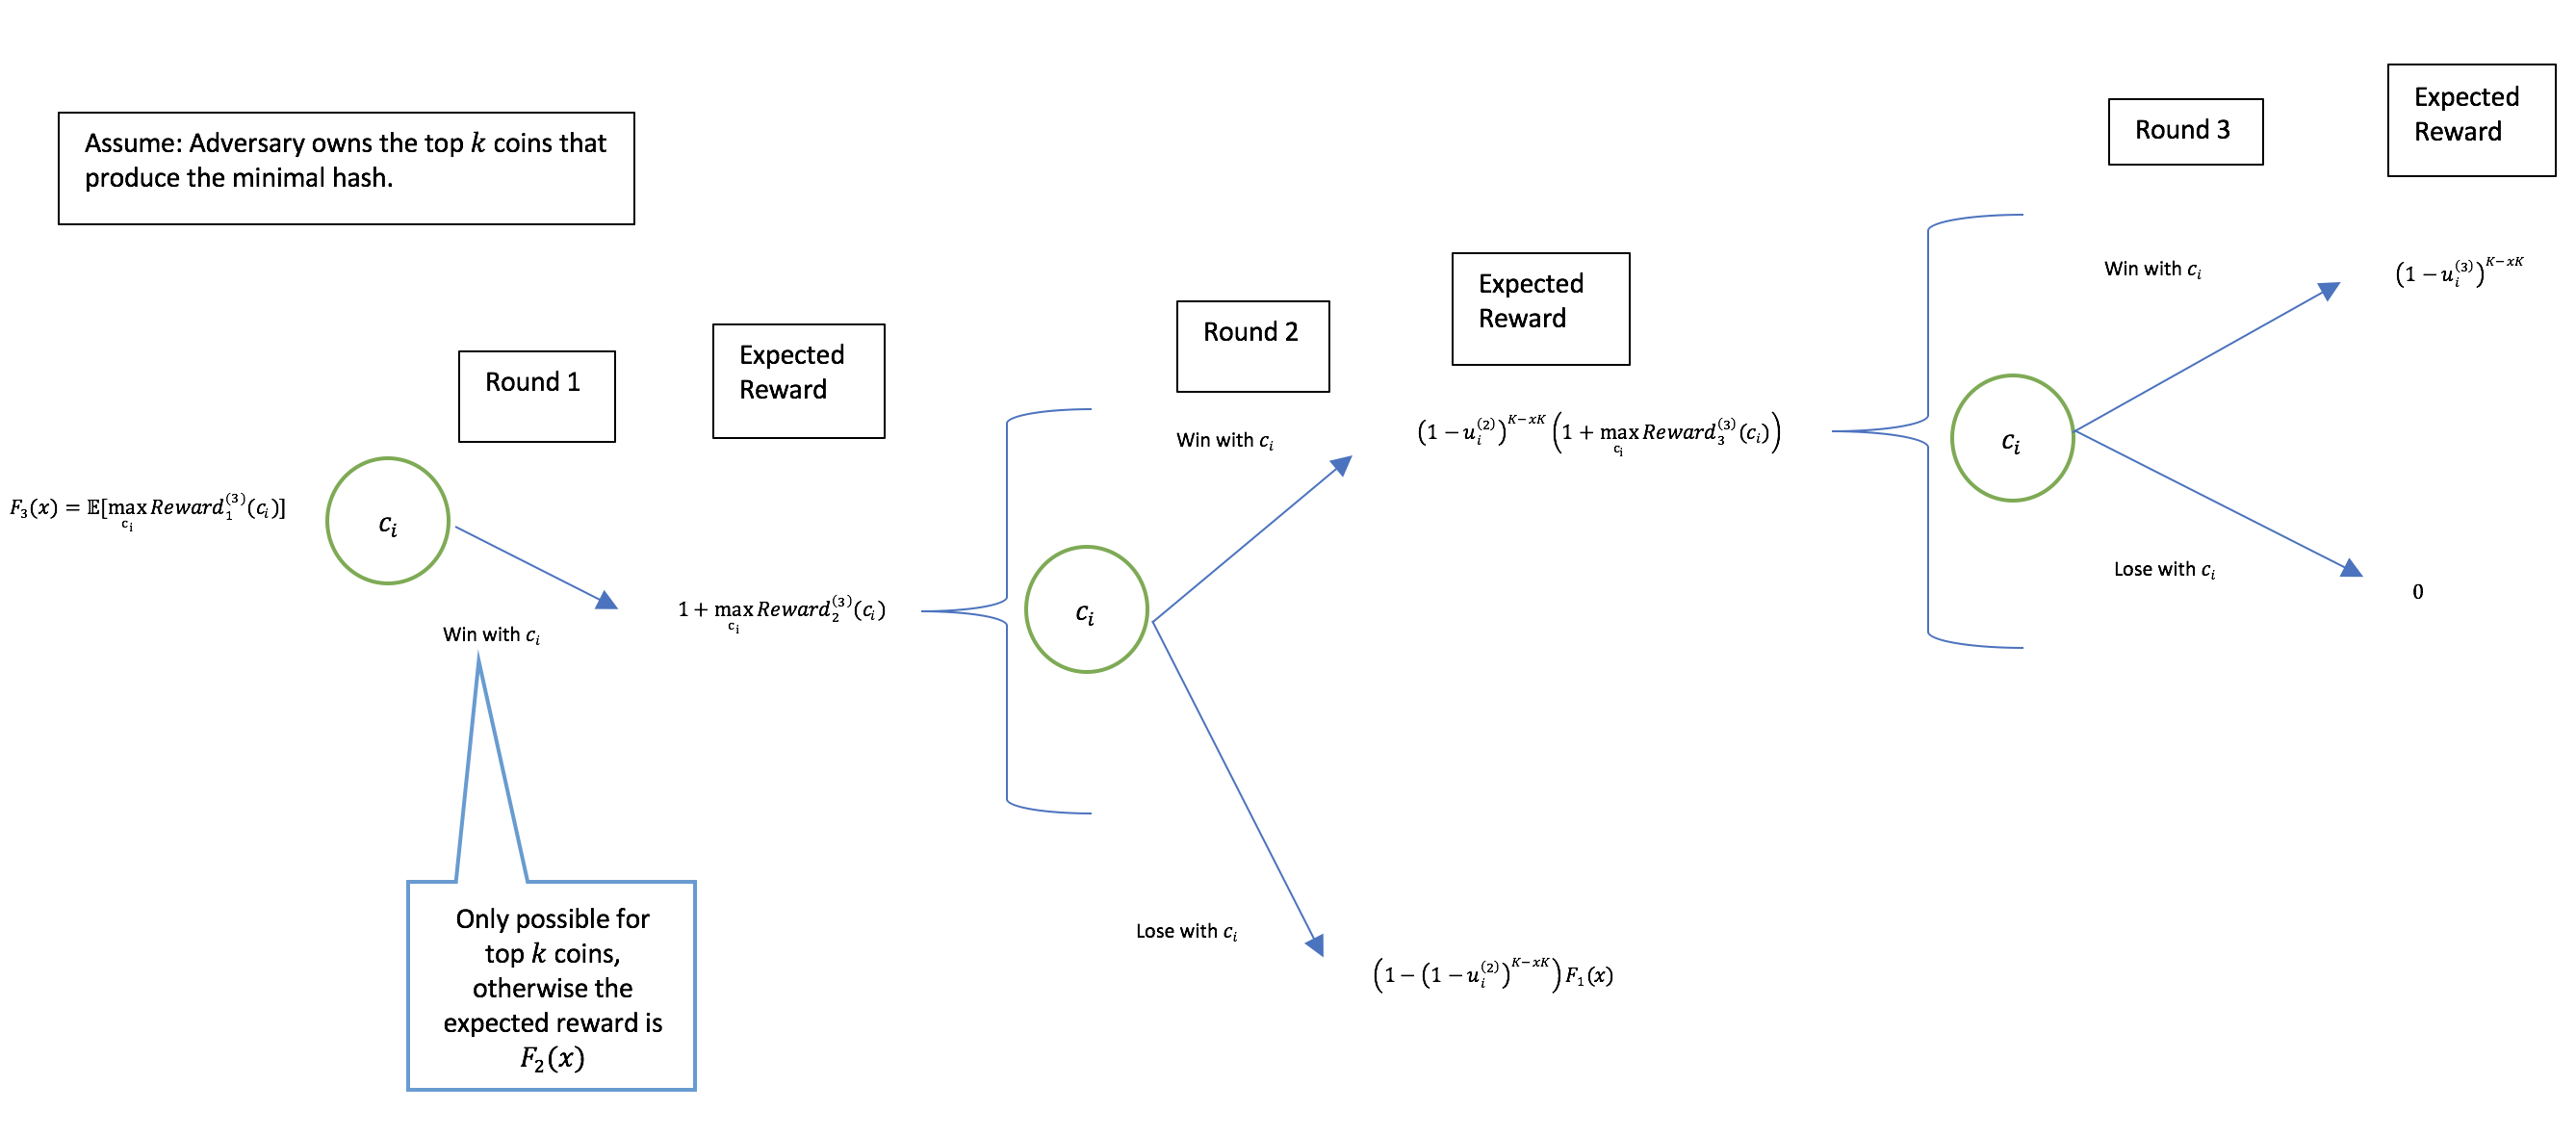
\includegraphics[width=1\textwidth]{decision_tree.png}
\caption{\label{fig:decision_tree}Decision tree that the adversary uses to maximize his expected total reward for a subgame with $n=3$ rounds.}
\end{figure}


\subsubsection{Analysis}
We can analyze the strategy as follows. See \ref{fig:decision_tree} for a diagram of an analysis of this approach for a 3 round subgame. Consider the adversary in round 1. The adversary can wait until the end of the transmission phase to know the hashes of all the other coins of other players, and therefore know exactly the rankings of his coins and knows deterministically whether he can win or lose in the next round for each of his coins. Let his coins be $\{c_i\}$. WLOG, say the adversary owns the top $k$ coins, then let these coins be $\{c_i\}_{i=1}^k$. Then if the adversary chooses to transmit coin $c_i$ from his top $k$ coins, then he will reap a reward of $1$ in round $1$ plus expected total reward of $Reward^{(3)}_2(c_i)$ in subsequent rounds. Otherwise, he can win an expected total reward of $F_2(x)$ if he chooses to transmit a losing coin or no coin at all because this essentially resets the game to a $2$ round subgame because he has no control of the seed for the next round and thus has no prior information about the hashes of his coins. So we have

$$
F_3(x) = \sum_{k=1}^{K} P_{k, x} \mathbb{E}\left[ \max\left\{1+\max_{c_i \in \text{Top k coins}} Reward^{(3)}_2(c_i), F_2(x) \right\}\right].
$$

The problem then becomes how to calculate $Reward^{(3)}_2(c_i)$. Now, since we are conditioning on the adversary winning in round $1$, the adversary can calculate the has of all his coins round $2$. Now, for each coin $c_i$, let the hash be $u_i^{(2)}$ in round $2$. Then we see that these hashes are uniformly and independently distributed on $[0,1]$, along with the hashes for each of the other coins that all the other players own. Thus, since coin $c_i$ wins the round if and only if its hash is the lowest, then the probability that coin $c_i$ wins in round $2$ is $(1-u^{(2)}_i)^{K-xK}$ since there are $K-xK$ other coins not owned by the adversary. In this case, the adversary reaps a reward of $1$ in round $2$ and then a expected reward of $Reward^{(3)}_3(c_i)$. If the adversary loses round, which occurs with probability $1-(1-u^{(2)}_i)^{K-xK}$, its expected total future reward is $F_1(x)$ because this essentially resets the game to a $1$ round subgame because he has no control of the seed for the next round and thus has no prior information about the hashes of his coins. The other choice for the adversary is to lose this round by not transmitting any coin (which may be the case if his expected future reward is low enough, which might occur if all his future hashes happen to be very large), and so this essentially resets the game as well and gives him an expected total return of $F_1(x)$. So we have

$$
Reward_2^{(3)}(c_i) = \max\left\{ (1-u^{(2)}_i)^{K-xK} \left(1+\max_{c_j}Reward^{(3)}_3(c_j)\right) + \left[1-(1-u^{(2)}_i)^{K-xK}\right]F_1(x), F_1(x)\right\}.
$$

Now that we are at the last round, we can calculate $Reward_3^{(3)}(c_i)$ immediately. That is, you win with coin $c_i$ with probability $(1-u^{(3)}_i)^{K-xK}$ and so the expected reward is

$$
Reward_3^{(3)}(c_j) = (1-u^{(3)}_j)^{K-xK}.
$$

Now, note that in the expression for $Reward_2^{(3)}(c_j)$, we are taking the maximum of $k$ randomly distributed variables and $F_2(x)$. This becomes like a dynamic programming problem, as we can calculate the numerical value for $F_i(x)$ for all $i<n$ compute the value of $F_n(x)$ from there.

\subsubsection{Some Computational Problems}
Now, since we are concerned with calculating $F_3(x)$, which involves the expectation of the maximum of $k$ random variables in each summand, and the distribution of these random variables is fairly complicated, we may have to rely on random simulation to calculate the expected values. It is unfortunate that there are no intermediate values like the $Reward^{(n)}_r$ functions that we can compute directly, because they are all random variables, and the expectation occurs outside of the $\max$ function.

\subsubsection{Next Steps}
\begin{itemize}
\item Confirm with professor Weinberg about the math behind this update.
\item Explore some options to see if we can calculate $F_n(x)$ without programmatically simulating the random variables or perhaps define a new metric for average reward reaped that may overcome this computational problem.
\item If there is no other way, then begin writing code to simulate the random variables programmatically.
\end{itemize}

\end{document}  